\chapter{Referencial Teórico}

\iffalse
\section{Qualidade de Software}


\section{Métricas de qualidade OO}

CKsuite
em quê foi baseado essas metrica.
quais são os métricas e como interpreta-las
\fi

\section{Princípios e Padrões de Projetos}

Desenvolver software orientado a objetos é um desafio. Criar uma representação
computacional de uma faceta da realidade em que seus constituintes trabalhem de
forma horminiosa para atingir as necessidades que o software se propõe a
atender requer experiência, conhecimento do domínio do problema e um processo de
análise e projeto. Apesear de existir várias abordagens para se conceber um
sistema orientado a objetos\cite{evans2004ddd},\cite{gomma11} um sistema bem
contruído apresetam características fundamentais. Coesão, acoplamento etc
\cite{demarco},\cite{page-jones}.


Um padrão dentro do contexto de estudo deste presente trablho pode ser definido
como uma técnica efetiva cuja a sua aplicabilidade é aceita e difundiida dentro
de uma área de conhecimento com a intenção de atingir um
objetivo\cite{MetskerWake06}.

Em densenvolvimento de software o catálogo mais difundido de padrões de projetos
orientado a objetos é elaborado por \citeonline{gof} contendo um total de 23
padrões formalmente documentados que acumulam experiências bem sucedidas 
diversos sistemas. Esses padrões tem a seguinte classificação:


\begin{description}
\item[Criacionais] Padrões que definem como criar novas instâncias de classes.
\item[Estruturais] Foca na estruturação das classes e objetos.
\item[Comportamentais] Definem como as classes e objetos interagem entre si e
suas responsabilidades.
\end{description}

Com o intuito de documentar os padrões de projetos de forma objetiva para
facilitar o aprendizado dos mesmos, a comparação e escolha do padrão a ser
aplicado, \citeonline{gof} elabora um modelo que descreve as seguintes
caracteristicas para cada padrão:

\begin{description}
\item[Nome e Classificação]
\item[Intenção]
\item[Também conhecido como]
\item[Motivação]
\item[Aplicabilidade]
\item[Estrutura]
\item[Participantes]
\item[Collaborations]
How the participants collaborate to carry out their responsibilities.
\item[Consequences]
How does the pattern support its objectives? What are the trade-offs and results
of using the pattern? What aspect of system structure does it let you vary inde-
pendently?
\item[Implementation]
What pitfalls, hints, or techniques should you be aware of when implementing
the pattern? Are there language-specific issues?
\item[Sample Code]
Code fragments that illustrate how you might implement the pattern in C++ or
Smalltalk.
\item[Known Uses]
Examples of the pattern found in real systems. We include at least two examples
from different domains.
\item[Related Patterns]
\end{description}

%argumentação
Analisando a forma como um padrão de projeto é concebido definindo papéis de
cada elemento participante e como eles interagem entre se podemos concluir que
os padrões de projeto promovem maior coesão, melhor separação de interesses e
baixo acoplamento no sistema.


\section{Model View Controller}

O padrão Model View Controller surgiu como uma solução genérica para usuários
de uma sistema de planejamento manipulem dados complexos\citeonline{Reenskaug:1979}.
Posteriormente \citeonline{krasnerPope1988} implementam um framework MVC para o
ambiente gráfico da linguagem de programação Smalltalk-80 como uma forma de
promover a reusabilidade e plugabilidade.

Segundo \citeonline{Reenskaug:1979} o principal objetivo do MVC ``\ldots was to
support the user's mental model of the relevant information space and to enable
the user to inspect and edit this information.''. Esse modelo mental é como o
usuário percebe o dominio do problema que está inserido no qual executará suas
atividades sobre dados de seu interesse. Para que o usuário de um sistema de
informação possa interagir com a represetação computacional  de seu modelo
mental três componetes são definidos:

Models - É o compoente constituído de uma composição de classes que implementam
as regras de negócio referentes as funcionalidades que o programa provê,
representa o  conhecimento que o usuário tem e como manipula-lo. Atende
mensagens da view requisitando seu estado e mensagens do controller para mudar
seu estado,

Views - Representação específica de um model na interface com o usuário, é 
responsável por todo a manipulação visual, recuperando um estado do model e
exibindo os dados, podendo ser composta por sub-views e ser parte de views mais
complexas.

Controllers - Interpreta a as ações do usuário provenientes de um dispositivo de
entrada(Teclado, Mouse) alterando estado da view ou do model.




\citeonline{krasnerPope1988} descreve a estrutura do MVC onde a view tem seu
controller exclusivo mantendo uma dependência cíclica entre ambos e tanto a view
quanto o controller tem referências diretas para o model por meio de atributos
de classe porém o model não deve conhecer seus respectivos pares de
View-Controller para promover mais reuso de código e encapsulamento do model. As
alterações do estado do model são feitas na maioria das vezes pelo controller, e
o model é responsável por notificar todas as views que o representa para que
se atualizem refletindo o novo estado. No caso de um model ser usado por vários
pares de View-Controller as mensagens de notificação de um novo estado do model
podem ser parametrizadas assim cada view pode verificar se a alteração é de seu
interesse. Segundo \citeonline{Fowler:2002:PEA} ``Of these the separation of presentation
from model is one of the most fundamental heuristics of good software design''.

O controller poderia ser o responsável por publicar as alterações no estado do
model devido sua relação direta com o mesmo, mas em casos onde o model é
alterado por outro componente que não é um dos controladores que os utilizam, é
necessário que o model conheça as views que devem ser notificados do novo
estado. Para que essas alterações de estado sejam propagadas a view e o
controller são registrados como dependentes de seu model. O padrão é descrito
dentro do contexto no qual o surgiu levando em consideração caracteristicas
espefíficas da  linguagem de programação que dão suporte à implementação dos
três componentes como por exemplo o gerenciamento dos objetos que são
dependentes do model definido na classe Objet que o model deve extender. A
Figura \ref{mvc_seq} esclarece a interação entre os componetes.

\begin{figure}[h]
	\centering
	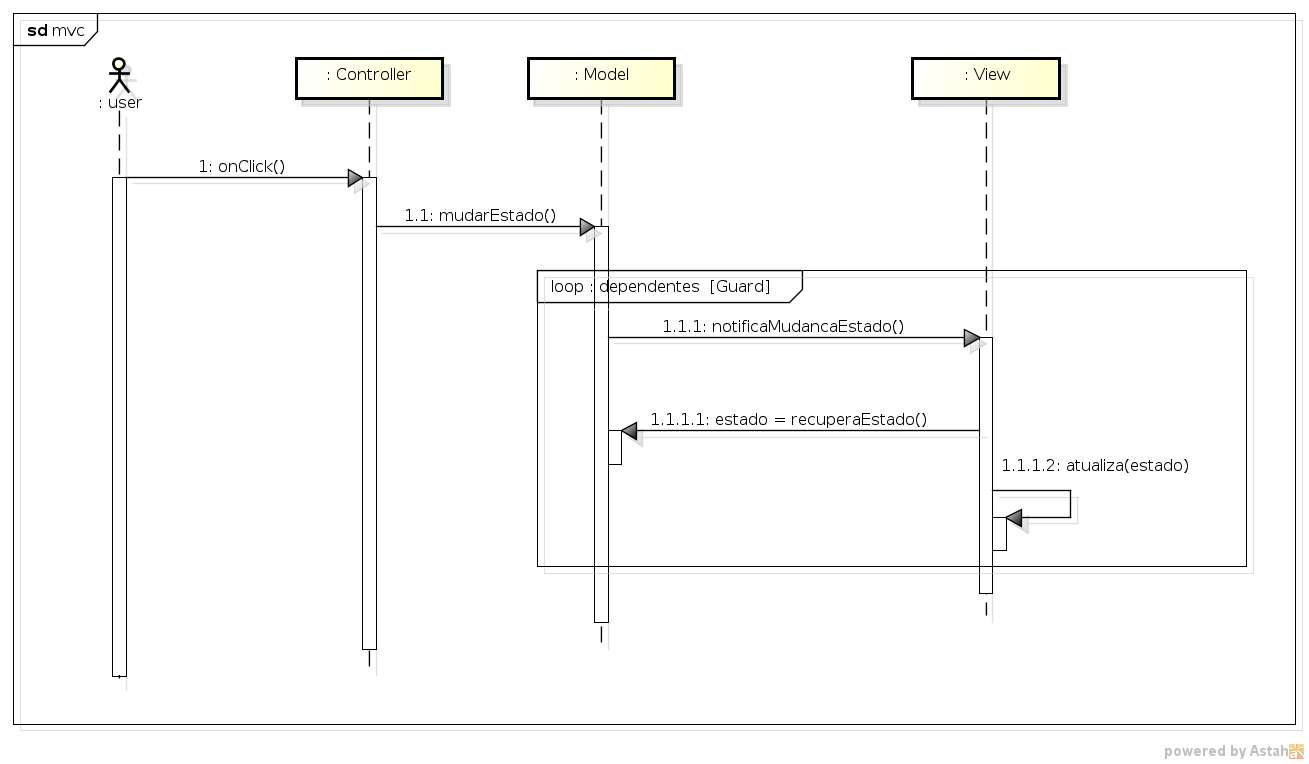
\includegraphics[scale=0.5]{img/mvc_seq.png}
	\caption{Diagrama de Sequência do MVC/Fonte: Próprio Autor}
	\label{mvc_seq}
\end{figure}

\citeonline{gof} cita \citeonline{krasnerPope1988} fazendo uma análise dos
objetos que compõem o MVC relacionando-os com outros padrões de proejtos. O
desacoplamento entre a view e o model e a propagação das mudanças de estado no
model para os objetos regitrados como dependentes do model pode ser descrico
como uma implementação do padrão Observer. A hierarquia de views é um exemplos
de Composite pois uma view pode ser constituída por sub-views para compor views
complexas. O Strategy é aplicando ao controller que encapsula o algoritmo que
vai alterar a view e o model podendo ser substituído por uma outra
implementação que deixa de responder às interações com o usuário.

Segundo \citeonline{krasnerPope1988} o Model ``\ldots can be as simple as an integer
(as the model of a counter) or string (as the model of a text editor), or it can
be a complex object''. O model pode ser implementado usando o pardrão Facade
para simplificar as interações com o model dependendo da complexidade do
domínio que ele representa.
%citar facade aqui



\section{Model View Presenter}

O MVP é um modelo de programação para implementação de interfaces com o usuário
desevolvido como um framework para C++ e Java, criado por uma subsidiária da IBM
chamda Taligent,Inc. Este padrão é baseado no MVC e descreve vários componentes que tem as
responsabilidades de como gerenciar os dados da aplicação e como o usuário
interage com esses dados tendo como objetivo promover o encapsulamento do Model
, reuso de lógica de negócio e o polimorfismo da View.

\begin{description}
  \item[Model] Tem as mesmas responsabilidades que o Model definido pelo MVC.
  \item[Selections] - Abstração para selecionar um subconjunto dos dados
  existentes no model.
  \item [Commands] Representa as operações a serem executadas sobre uma
  Selection do Model.
  \item [View] Responsável por exibir o model assim como no MVC.
  \item [Interactor] Mapeia os interações do usuário na view como eventos do
  mouse.
  \item [Presenter] O papel do presenter é interpretar o eventos iniciados pelo
  usuário executando a lógica de negócio correspondente implementada em um
  command para manipular o model \cite{Potel96mvp}.
\end{description}


%interpretações do mvp
%Objectarts
Os conceitos do MVP são descritos em \citeonline{Potel96mvp} de forma genérica
permintindo interpretações para uma implementação efetiva.
\citeonline{twisttriad:2000} descreve a implementação de um framework para
Dolphin Smalltalk\footnote{Implementação da Linguagem de programação Smalltalk,
http://www.object-arts.com} adotando os conceitos do MVP onde salienta que a
maioria dos sistemas operacionais com ambiente gráfico fornece um conjunto de
componetes (Widgets) no qual está contido a responsbilidade do controller.A
maior parte do comportamento do caso com o usuário é implementada no
presenter que está diretamente associado a View

Ainda acerca das responsabilidades do presenter \citeonline{fowler:ui} descreve
o que é chamado de Passive View onde toda a lógica do comportamento da view é
implementado no presenter deixando a view enxuta com o intuito de isolar ao
máximo a api gráfica do resto da aplicação, permitindo uma maior cobertura de
testes aplicados ao presenter. Dessa forma o model não se comunica com a view
por meio do observer pattern, sendo que a view séra atualizada pelo presenter.


discorrer sobre a interpretação de An Architecture and Implement Model for
Model-View-Presenter Pattern

%Conclusão


MVP se adequa melhor as apis gráficas existentes. Define de forma mais clara os
componetes necessários para desenvolver uma aplicação, sendo o ponto de maior
discussão reside em quais os limites das responsabilidades no que tange a
mediação do Model e a View.


\section{Framework Android}
 
Historia caracteristicas
Arquitetura.

Componentes
	Activity
	service
	broadcastReceiver
	ContentProvider



Como DP resolvem problemas, seguir linha de raciocinio para aplicar padrões em
android.


Analise do componente Activity, UI Thread, hieráriquia de herança e algumas
funcionalidades que dependem da activity e como isso interfere na aplicação do
padrão(Por experiência confirmo que é negativa). mostrar exemplo de uma view em
lista para smartphone e outra para tablet com grid usando o mesmo modelo

Experimentos

activity - controller+async task - listeners,
activity - controller+async task - observer pattern,
activity - controller+async task - localbroadcast
activity - controller+async task - Messages
Activity+Fragment


\citeonline{Reenskaug:1979} The View and Controller roles may be played by the 
same object when they are very tightly coupled. Example: A Menu., porém isso
requer um boa análise do problema em questão para decidir o nível de
granularidade que esses componentes podem ter portanto é recomendável manter
sempre essa separação.É aplicável para 


